\documentclass{standalone}
\usepackage{tikz}
\usepackage{pgfplots}

\begin{document}

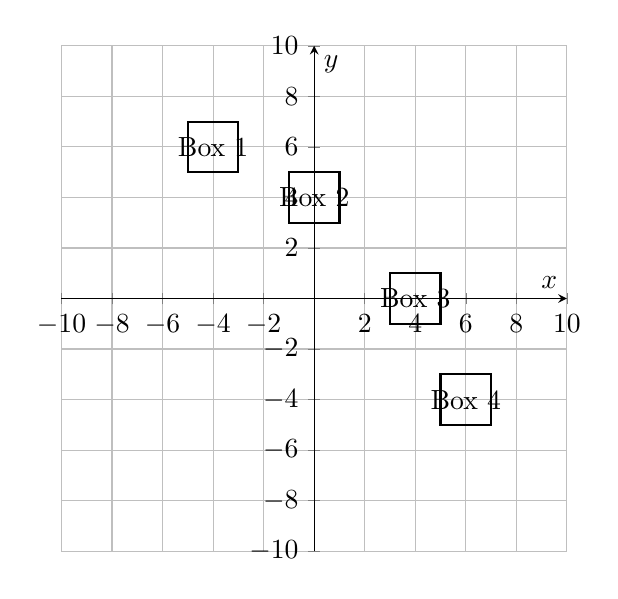
\begin{tikzpicture}
    % Define the coordinate system
    \begin{axis}[
        axis lines=middle,
        xlabel=$x$,
        ylabel=$y$,
        xmin=-10,
        xmax=10,
        ymin=-10,
        ymax=10,
        xtick distance=2,
        ytick distance=2,
        grid=major,
        width=8cm,
        height=8cm,
        enlargelimits=false
    ]
        
        % Draw the first box
        \draw[thick] (axis cs: -5, 5) rectangle node[pos=0.5] {Box 1} (-3, 7);
        
        % Draw the second box
        \draw[thick] (axis cs: -1, 3) rectangle node[pos=0.5] {Box 2} (1, 5);
        
        % Draw the third box
        \draw[thick] (axis cs: 3, -1) rectangle node[pos=0.5] {Box 3} (5, 1);
        
        % Draw the fourth box
        \draw[thick] (axis cs: 5, -5) rectangle node[pos=0.5] {Box 4} (7, -3);
        
    \end{axis}
\end{tikzpicture}

\end{document}